\documentclass[12pt]{article}

%
%Margin - 1 inch on all sides
%
\usepackage[letterpaper]{geometry}
% \usepackage{times}
\usepackage{mathpazo}
\usepackage{amssymb}
\usepackage{listings}
\usepackage{xcolor}
\usepackage{graphicx}

\definecolor{codegreen}{rgb}{0,0.6,0}
\definecolor{codegray}{rgb}{0.5,0.5,0.5}
\definecolor{codepurple}{rgb}{0.58,0,0.82}
\definecolor{backcolour}{rgb}{0.95,0.95,0.92}

\lstdefinestyle{mystyle}{
    backgroundcolor=\color{backcolour},   
    commentstyle=\color{codegreen},
    keywordstyle=\color{magenta},
    numberstyle=\tiny\color{codegray},
    stringstyle=\color{codepurple},
    basicstyle=\ttfamily\small,
    breakatwhitespace=false,         
    breaklines=true,                 
    captionpos=b,                    
    keepspaces=true,                 
    numbers=left,                    
    numbersep=5pt,                  
    showspaces=false,                
    showstringspaces=false,
    showtabs=false,                  
    tabsize=2
}
\usepackage{minted}
\lstset{style=mystyle}

\geometry{top=1.0in, bottom=1.0in, left=1.0in, right=1.0in}

%
%Doublespacing
%
\usepackage{setspace}


%
%Fancy-header package to modify header/page numbering (insert last name)
%
\usepackage{fancyhdr}
\usepackage{ragged2e}
\usepackage{indentfirst}
\usepackage{sectsty}
\sectionfont{\normalfont\normalsize\bf}
\subsectionfont{\normalfont\normalsize\it}
\subsubsectionfont{\normalfont\normalsize\it}
\pagestyle{fancy}
\usepackage[backend=bibtex]{biblatex-chicago}
\lhead{}
\chead{} 
\rhead{}
\lfoot{} 
% \cfoot{$\cdot$ \hspace{.4em} \thepage \hspace{.4em} $\cdot$ } 
\cfoot{\thepage}
\rfoot{} 
\renewcommand{\headrulewidth}{0pt} 
\renewcommand{\footrulewidth}{0pt} 
\newcommand{\wordcount}{400} 
%To make sure we actually have header 0.5in away from top edge
%12pt is one-sixth of an inch. Subtract this from 0.5in to get headsep value
\setlength\headsep{0.333in}

%
%Works cited environment
%(to start, use \begin{workscited...}, each entry preceded by \bibent)
% - from Ryan Alcock's MLA style file
%
\newcommand{\bibent}{\noindent \hangindent 40pt}
\renewcommand{\part}[1]{{\center \sc #1}}
\newenvironment{workscited}{\newpage \begin{center} References \end{center}}{\newpage }

\bibliography{paper}

%
%Begin document
%
\begin{document}

	%%%%First page name, class, etc

	%%%%Title
	\begin{center}
		\textbf{In-dex}

		\emph{Varun Iyer} \hspace{.34em}$\cdot$\hspace{.34em} \emph{2014 words}
	\end{center}
	\par

	\begin{abstract}
		This paper introduces in-dex, a tool that creates cross-reference links
		to important phrases within documents. The first section contextualizes
		the tool’s function and purpose. The second section describes the tool
		itself. The third section discusses the implementation and technical
		aspects of in-dex.
	\end{abstract}

	\section{Background}

	Most written works in English are meant to be read top to bottom.
	Authors must wrangle complex ideas into linear form, so that they can be
	understood in series by the reader.

	Some works stand as exceptions to this rule --- for example, branching
	narrative stories, or reference works that are meant to be read one entry
	at a time as necessary.

	Digital works push the envelope by generating connections between different
	pieces of text in ways that the author did not explicitly specify. For
	example, Zoe Quinn’s Depression Quest guides the user through a narrative
	that changes depending on the player’s choices, and has many different
	possible ways to play through it, not all of which were explicitly laid out
	by the author.\autocite{dq}

	As another example, Wikipedia creates cross-references between different
	articles depending on the words used in a given article. This connects
	articles together into graphs that can be explored by a person, jumping
	from link to link, or by software that analyzes the relationships between
	articles.\autocite{wiki} These connections allow readers to read the text
	of Wikipedia in non-linear, unintended ways.

	Code is also a unique kind of written artifact that is often read ‘out of
	order.’ Code is not read in order of writing, in the order it falls on
	the page, or in order of execution. Rather, it is read in a reverse-climax
	order, from broadest and boldest strokes down towards the details that a
	specific programmer is interested in.\autocite[140]{brock}

	I was inspired to make in-dex by the way that indexing works in traditional
	non-fiction works and unintentional cross-referencing and network creation
	on digital platforms like Wikipedia. In-dex identifies important, key
	phrases in a traditional, linear text and then hyperlinks together
	successive uses of the phrase. This creates in-text cross references. By
	clicking a hyperlink, a user can jump to the previous or next use of a key
	phrase. The aim of these connections is to allow a user to explore a
	document in a non-linear way.

	This non-linear exploration is a common strategy used to build an
	understanding of an area that cannot be read cover-to-cover, so to speak.
	For example, the U.S. legal corpus is far too large for single person to
	comprehend. If a person seeks to understand an area of the law, they have
	two choices. First, they could refer to a casebook, a representative set of
	documents curated and organized by an expert in the field.\autocite{lil}
	Or, they could identify cases they think are important and read other works
	that the original case relies on heavily and future works that rely on the
	original case --- constructing a casebook of sorts by using the information
	already available within the text. This process is similar to the ‘relevant
	content’ suggestions generated by social media platforms.\autocite{pixie}

	I have been exploring academic and legal content suggestion recently
	through a project called Lexcaliber.\autocite{lex} In-dex applies network
	exploration of text to navigation in a single document, rather than in a
	body of works.

	A user who jumps from phrase to phrase explores a document by the ways that
	it touches on a particular topic, potentially revealing relationships or
	narratives that are more difficult to uncover when reading a document in
	its intended fashion. I have found in-dex especially helpful in exploring
	complex documents such as court opinions, as they touch on many different
	issues in different parts of the document. Cross-referencing works
	particularly well in allowing reading one issue at a time.

	\section{Description}

	The functionality of in-dex is currently as follows: the in-dex program is
	run with a simple HTML file (for example, the kind produced by Firefox
	reader) as an input. The program writes an indexed HTML file that contains
	links between key phrases in the original HTML file. This file can then be
	opened in any browser and the links can be explored.

	The text of such a file is picture in Fig. \ref{html}, with in-dex’s output
	pictured in Fig. \ref{idx}. In-dex inserts small arrows linking important
	terms together --- in this case, ‘installation of pen register’, ‘search of
	petitioner’s residence,’ and ‘Court of Appeals of Maryland,’ among other
	terms. The up arrow carries the user to the previous use of the phrase,
	while the down arrow carries the user to the next use of the phrase.

	The interface of in-dex is minimal, leaving the text of the document
	unobstructed and still dominating the uesr’s view.

	\begin{figure}[h]
		\center
		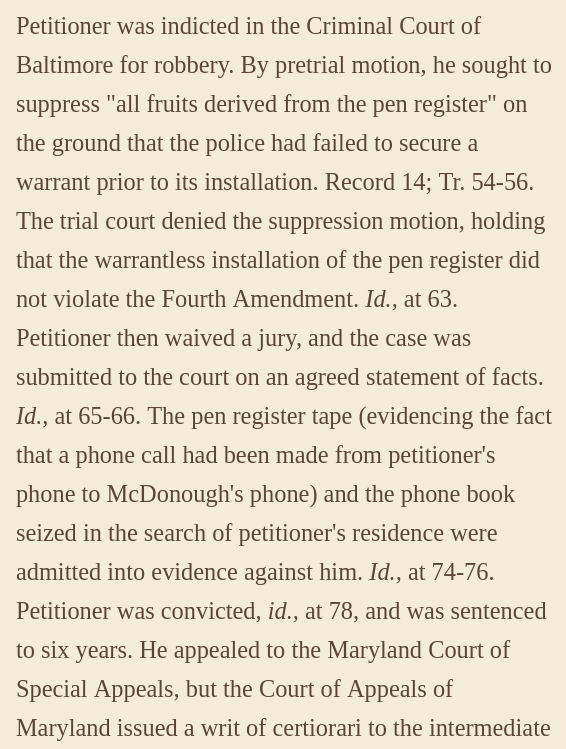
\includegraphics[width=0.6\textwidth]{html.png}
		\caption{Original text of \emph{Smith v. Maryland}\autocite{smith}}
		\label{html}
	\end{figure}
	\begin{figure}[h]
		\center
		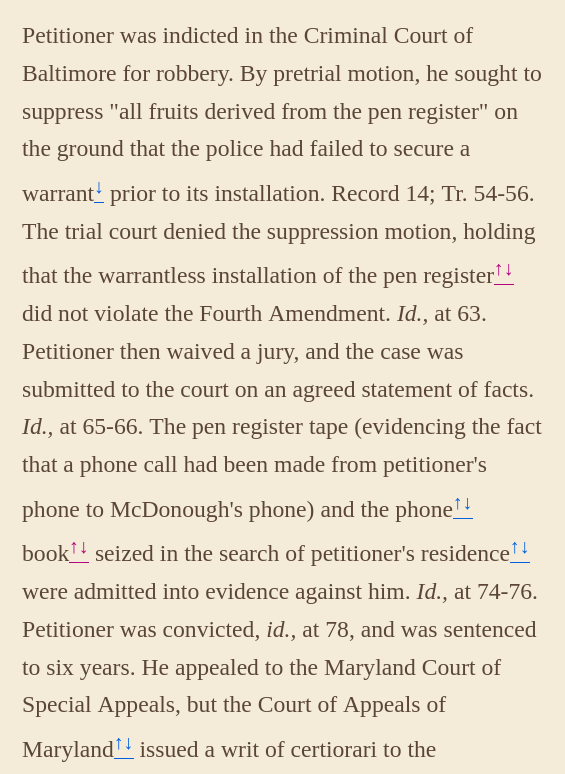
\includegraphics[width=0.6\textwidth]{idx.png}
		\caption{\emph{Smith v. Maryland}\autocite{smith} after markup by in-dex; note the small arrow links after several terms.}
		\label{idx}
	\end{figure}
		

	\section{Tech}

	While having a relatively simple functionality, the working of in-dex is
	somewhat complicated, involving six distinct steps. I’ll describe the
	steps and then explore the most important steps in greater detail.
	 
	\begin{enumerate}
		\item Tokenize raw text into constituent sentences and words, and
			exclude stop words.
		\item Count occurrences of phrases bundles of 3-4 sentences.
		\item Identify phrases that occur in multiple bundles and multiple times
			in each bundle (suggesting a paragraph that deals with a given topic).
		\item Fuzzy-find all occurrences of such key phrases in the document.
		\item Insert HTML markup to identify these phrases.
		\item Insert links that jump from one phrase occurrence to the next.
	\end{enumerate}

	After identifying the words present in the document, in-dex must determine
	which concepts are relevant or important to the document. Finding a
	heuristic to approximate significance is a non-trivial problem, and
	required a few different attempts to identify a solution that seemed to
	work.

	A first attempt relied on sent2vec, an unsupervised natural sentence
	vectorizer closely based on the famous word2vec. A vectorizer like sent2vec
	uses machine learning or traditional techniques to numerically represent
	non-quantitative data.\autocite{s2v} While this method had some success in
	identifying semantically similar sentences, it was not very effective at
	determining which of these relationships are significant or helpful.

	Ultimately, the most effective method was a unique approach combining
	two different techniques, n-gram analysis and tf-idf. N-gram analysis is a
	method of text analysis that takes sequences of words rather than
	individual words as its fundamental unit of analysis. Looking at pairs or
	three words used adjacent to each other proved effective because identical,
	repeated phrasing is a good indicator that the same concept or topic is
	being discussed. Tf-idf is a technique used to identify relevant or
	interesting objects by analyzing the frequency of their
	occurence.\autocite{tfidf} Terms that occur many times in one document (or
	paragraph, or set of sentences) but that do not occur in many documents are
	likely good descriptors of the unique content of that document. I applied
	the tf-idf counting method to series of three words, which proved to be
	effective at identifying recurring themes or topics unique to a few
	different parts of a text.

	Figuring out how to represent the connections between different sections
	proved to be quite difficult; ultimately, I decided that displaying all
	possible connections was too visually cluttering and functionally
	confusing. Instead, the tool currently allows the user to jump to the
	previous use of a phrase (by clicking the 'up' arrow link) or the next use
	(by clicking the 'down' arrow link). Ultimately, in-dex still relies on
	the linear orientation of the original document, but allows different ways
	to move across it.

	\section{Conclusion}

	Digital technology and repositories of text open up new possibilities for
	how that text can be presented, read, shared, and explored.  In-dex is a
	small proof-of-concept for a tool that allows users to navigate complex
	documents in non-linear ways. However, the true benefit of a tool like
	in-dex will likely be revealed more clearly when dealing with groups of
	documents rather than cross-referencing a single document. While in-dexing
	a single document is an interesting curiosity, in-dexing a set of complex
	documents may allow readers to identify connections in text that would have
	otherwise gone unnoticed. I hope to expand in-dex to fulfill this purpose
	in the near future.

	\printbibliography

\end{document}
